\documentclass[UTF8]{ctexart}
\usepackage{geometry}
\usepackage{xcolor}
\usepackage{pgf-pie} % the package used to implement the pie charts
\usepackage[pdf]{graphviz}

\begin{document}
\Huge boggy chicken \small

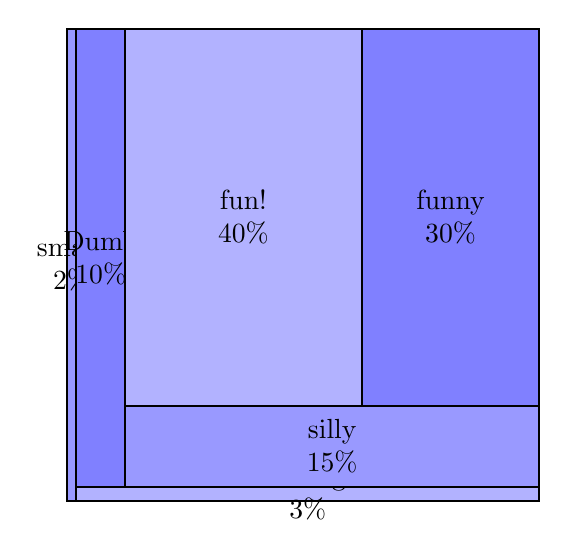
\begin{tikzpicture} % Tikz environment
\pie [square, text=inside, color={blue!40, blue!30, blue!50} ]
 {2/smart, 3/strong, 10/Dumb, 15/silly, 40/fun!, 30/funny} 

 % it is essential to recheck that the sum of all the components mentioned should be 100%. Otherwise, Latex will leave the left percentage, blank.
\end{tikzpicture}


\Huge boggy bird \small
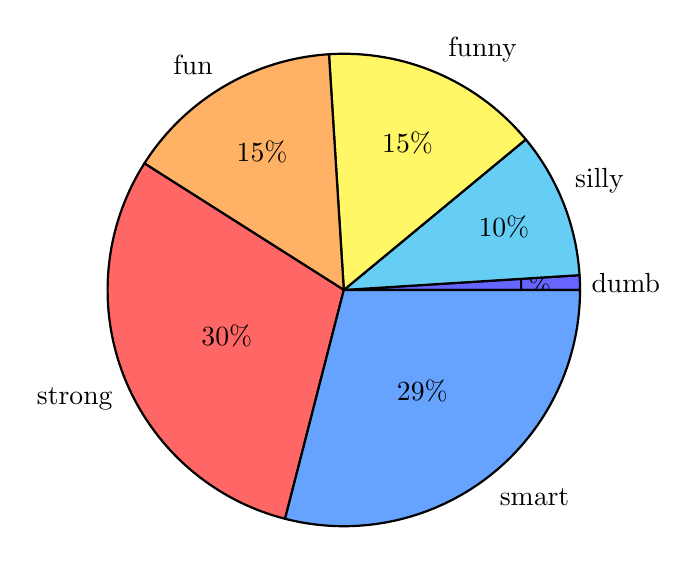
\begin{tikzpicture}
\pie  {1/dumb, 10/silly, 15/funny, 15/fun, 30/strong, 29/smart}
\end{tikzpicture}


\digraph{abc}{
   rankdir=LR;
   a -> b -> c;
}

\end{document}
